

\tikzset{every picture/.style={line width=0.75pt}} %set default line width to 0.75pt        

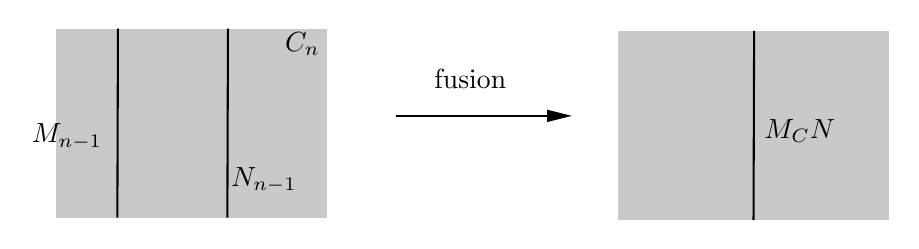
\begin{tikzpicture}[x=0.75pt,y=0.75pt,yscale=-1,xscale=1]
%uncomment if require: \path (0,300); %set diagram left start at 0, and has height of 300

%Shape: Rectangle [id:dp05644707403398308] 
\draw  [draw opacity=0][fill={rgb, 255:red, 0; green, 0; blue, 0 }  ,fill opacity=0.21 ] (91,36) -- (221.71,36) -- (221.71,127.06) -- (91,127.06) -- cycle ;
%Straight Lines [id:da16260553950193857] 
\draw    (121,36) -- (120.71,127.06) ;
%Straight Lines [id:da20481776934772644] 
\draw    (174,36) -- (173.71,127.06) ;
%Straight Lines [id:da43444643961615803] 
\draw    (255,78) -- (337.71,78) ;
\draw [shift={(339.71,78)}, rotate = 180] [fill={rgb, 255:red, 0; green, 0; blue, 0 }  ][line width=0.08]  [draw opacity=0] (12,-3) -- (0,0) -- (12,3) -- cycle    ;
%Shape: Rectangle [id:dp5696175787392299] 
\draw  [draw opacity=0][fill={rgb, 255:red, 0; green, 0; blue, 0 }  ,fill opacity=0.21 ] (362,37) -- (492.71,37) -- (492.71,128.06) -- (362,128.06) -- cycle ;
%Straight Lines [id:da7613999267121918] 
\draw    (427.5,37) -- (427.21,128.06) ;

% Text Node
\draw (200,36.4) node [anchor=north west][inner sep=0.75pt]    {$C_{n}$};
% Text Node
\draw (78,80.4) node [anchor=north west][inner sep=0.75pt]    {$M_{n-1}$};
% Text Node
\draw (174,101.4) node [anchor=north west][inner sep=0.75pt]    {$N_{n-1}$};
% Text Node
\draw (272,54) node [anchor=north west][inner sep=0.75pt]   [align=left] {fusion};
% Text Node
\draw (431,78.4) node [anchor=north west][inner sep=0.75pt]    {$M\boxtimes _{C} N$};


\end{tikzpicture}
